\section[Características de SuperCollider]{Características importantes y limitaciones de SuperCollider}
\sectionmark{Características de Supercollider}
\label{sec:sc_features}

\subsection{Orden de ejecución en el servidor}
En un sintetizador modular analógico no hay limitación alguna en el orden en el que se conecta sus módulos. Todos son independientes entre sí ya que se <<ejecutan>> al mismo tiempo. Cualquier señal de salida puede ser conectada a cualquier entrada. Esta es una de las características más interesantes y sugerentes de estos sintetizadores. En el manual de instrucciones de EMS Synthi VCS3 --antecesor del Synthi 100 y de características muy similares-- se invita al usuario a experimentar libremente con cualquier conexión. La posibilidad de que todo pueda ser conectado con todo hace de los sintetizadores modulares en general, y de los Synthi en particular, un banco de experimentación sonora sin precedentes.

Los sistemas informáticos actuales son multihilo, es decir, pueden ejecutar varias tareas a la vez. El tiempo de ejecución es repartido en todas ellas a velocidad suficiente como para crear en el usuario la ilusión de que ocurren las tareas simultáneamente, cuando en realidad solo una se lleva a cabo en un instante concreto. Los sintetizadores digitales aprovechan esta característica, pero sus módulos no se ejecutan simultáneamente, sino que siguen un orden preciso de ejecución entre ellos. En el caso de SuperCollider, cada \texttt{Synth} en el servidor ocupa un lugar en una lista, la cual es ejecutada en orden a la frecuencia de audio (\textit{audio rate}). Puesto que todos los módulos de \appName están construidos a base de \textit{Synths}, no será raro que la salida de uno de ellos sea conectada a la entrada de otro que ya ha sido ejecutado en el ciclo presente. Puesto que el contenido de los \textit{busses} de audio es eliminado al terminar un ciclo completo, la consecuencia es que ninguna señal llegará al módulo de destino. La figura \ref{fig:sc_server} representa esta característica unidireccional en el orden de ejecución de los nodos presentes en el servidor. Ningún \texttt{Synth} podrá enviar señal alguna a otro situado a su izquierda (el orden de ejecución es de izquierda a derecha en esta representación).

\begin{figure}
	\centering
	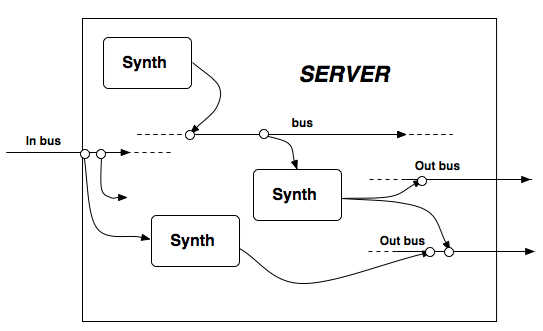
\includegraphics[width=0.7\textwidth]{images/sc_server}
	\caption[Orden de ejecución en el servidor de SuperCollider]{Orden de ejecución en el servidor de SuperCollider. Cada ciclo de audio los \texttt{Synths} presentes en el servidor son ejecutados en orden (de izquierda a derecha en esta respresentación). Ninguna información puede viajar por los \textit{busses} en sentido contrario, ya que su contenido es eliminado tras la finalización de cada ciclo.}
	\label{fig:sc_server}
\end{figure}

Existe un \textit{UGen} que permite obtener información de ciclos pasados de los \textit{busses}. Se trata de \texttt{InFeedback.ar()}. La limitación frente a \texttt{In.ar} es que la señal que recibe es la correspondiente a un ciclo de control previo. Aunque en la mayoría de los casos esto no tiene mayor importancia, es una característica importante a tener en cuenta, especialmente cuando se produce un \textit{feedback} en la señal, ya que su comportamiento distará mucho del que puede tener un sistema completamente analógico. 

\subsection{\textit{Audio rate} y \textit{control rate}}
No todo ocurre a la misma velocidad en SuperCollider. La producción de señales de audio requiere de la creación de un número de muestras por segundo igual a la <<tasa de audio>>. Pero no siempre es necesaria una demanda tan alta de computación. En el caso de los efectos como curvas relativamente lentas en los cambios de los parámetros sonoros pueden realizarse con una tasa mucho menor. Por ejemplo, un \textit{glissando} frecuencial de un segundo de duración entre 100 Hz y 1000 Hz, no necesita tener una resolución similar a la <<tasa de audio>>. Es posible realizarlo a una tasa (<<de control>>) bastantes veces menor a la de audio sin verse afectado auditivamente el resultado sonoro. Por defecto, la tasa de control en SuperCollider es 64 veces menor que la de audio.

Existe una clara analogía entre una señal de audio analógica y \textit{audio rate}, así como entre una señal de voltaje y \textit{control rate}. En una primera aproximación, podría parecer obvio que las señales de voltaje del Synthi 100 pueden ser emuladas digitalmente a la tasa de control. El problema de una decisión así es que limita considerablemente el uso que podemos hacer con esta señales <<de control>>. En un sintetizador analógico, una señal de control de voltaje puede ser utilizada como señal de audio y viceversa. No hay ninguna diferencia real entre ambos tipos de señal, más allá de una división puramente funcional. No hay ninguna razón que nos obligue a limitar las compotentes frecuenciales de una señal de voltaje en un sintetizador analógico. Por esta razón, \appName\ prescinde por completo de las señales en <<tasa de control>>. Todas las señales en la aplicación son del mismo tipo, con <<tasa de audio>>. Esto es posible, evidentemente, gracias a la capacidad de computación de los ordenadores modernos. A cambio de eficiencia se gana en versatilidad y, por supuesto, en aproximación al funcionamiento de un sintetizador modular.


\subsection{Los \texttt{Synths} ocupan recursos...}
Puede resultar una obviedad decir que tanto los \texttt{Synths} como los \textit{busses} digitales ocupan memoria y tiempo de ejecución, pero cuando estos elementos se empiezan a contar por miles, como en el caso de \appName, este es un factor que puede comprometer la eficiencia y la escalabilidad de la aplicación.



